%!TEX root = main.tex

\section{Architectures}
Classical games like chess or tic-tac-toe are usually ``solved'' by AIs using a
single approach and searching through a single tree of game states, though
usually by optimizing the search and tree in various ways.

In comparison most approaches to AIs playing real-time strategy games usually
have to use domain knowledge do further subdivide the problem of playing the
game, because of the fine-grained simulations involved, and the various levels
of abstraction that is needed to get a successful AI. And especially when
approaching the way humans think about a problem more complex architectures
are needed.

\subsection{Decomposition of problem}
Michael Buro in his 2003 call for research \cite{buro2003real} identified six
important sub-problems in real-time strategy games that he said would be
interesting for AI research to focus on:

\begin{description}
  \item [Resource management.] To be able to build up an army one needs to gather
    resources, and the balance between gathering resources (by creating workers),
    building an army and evolving through the technology tree is an important
    part of the macro/high-level strategy.
  \item [Decision making with uncertainty.] Because of fog of war, there is a
    high degree of uncertainty involved in the decision making. Therefore the AI
    needs to create hypotheses and act according to them, and should scout to
    confirm these.
  \item [Spatial and temporal reasoning.] Analyzing and predicting spatially as
    well as temporarily. Identifying choke points and predicting outcomes and
    utilities of actions it takes are some obvious applications.
  \item [Collaboration.] In most RTSes it is possible for players to ally, and
    how to share intelligence and coordinate attacks is a challenging problem,
    though maybe not as interesting yet.
  \item [Opponent modelling.] Learning from the opponent is an important skill,
    and exploting the weaknesses of your opponent is an important aspect of
    human-level playing.
  \item [Adverserial real-time planning.] Abstracting away micro-level
    management to allow for more efficient search in the game state-space, and
    translate the found solutions back, is an important problem to solve.
\end{description}

A lot of research as been done into AIs for RTSes since this, however, and the
list might be a bit outdated. For example, one important aspect of most AIs
today is the micro-management of units, trying to maximize the utility of them 
(maximizing output of resource gatherers and damage dealt by offensive units,
for example).

Another important problem that is under-valued by the above list is learning
from existing knowledge, like learning build-orders from replays of games played
by humans (or other bots, though the utility of that might not be substantial).
This can be integrated into several of the items above, for example the decision
with uncertainty by statistically inferring the most probable states by
learning from earlier games.

A more general and simplified breakdown of the problem of playing Starcraft can
be found in Ben Weber's presentation from the AIIDE 2010 StarCraft AI
Competition:\cite{weber2010aiide}

\begin{description}
  \item [Managing economy] is the same as the resource management mentioned
    above, and is about getting a steady income.
  \item [Expanding the tech tree] to get more powerful and varied units.
  \item [Producing units] is perhaps one of the most complex parts. This
    involves both buildings and movable units, defensive and offensive.
  \item [Attack opponent] usually is not a very explicit action, but can still
    be pretty complex, since one needs to evaluate its own state against what
    it knows about the opponent to know when to attack, and where. This point
    also involves micro-management, which has received a lot of attention from 
    authors of AIs that have ranked highly.
\end{description}

Solving all of the aforementioned problems by themselves are what is the focus
of most research today, but another important problem is tying all of these
solutions together again. This is perhaps one of the most basic, but important,
aspects of the architecture. There are several different ways of doing this,
and some of the most common one is simply sharing a large amount of information
between sub-units in the architecture (for example a black-board based
architecture), or simply having a well-defined graph hierarchy where decisions
are propagated.

\subsection{Hierarchical architectures}
Hierarchical architectures rely on one or more levels of subsumption of
responsibility in a hierarchy of modules to tie together the various partial
solutions to the sub-problems stated earlier.

\subsubsection{BTHAI}
BTHAI utilizes a multi-agent approach to create a system with high levels of modularity. Each unit and building is represented as an agent that extends a more general version of that agent type. So every building is a subclass of a structurAgent, and every unit is a subclass of an unitAgent. These again extend a baseAgent, and this creates a hierarchic structure where agents of a similar type can share logic for behavior and strategy, but supports the option of extending the agent in order to customize and specialize the behavior of that specific agent. 

For higher level tasks with as tactics, exploration and building the bot uses managers. The managers maintains all the agent objects for the different units that the bot controls. Managers also act as an information provider for the agents so they can access data and statistics about the current state of the game. For instance how many units that an attacking force consists of, and how many are defending the base etc. 
There are also an exploration manager, that handles everything related to exploration, where enemy units have been discovered and predictions about where they will move. A build planer decides what order buildings will be constructed in, and squad commanders handles higher level tactics for a group of units, like attacking or retreating. These managers also have an hierarchic structure, so that they can be extended in order to create a more specialized manager, like a race specific build planer. 

The creation of agent instances are the responsibility of an AgentFactory. This factory makes sure that the correct agent is created for a given unit and that if there exists a specialized agent type for that unit the correct one is created and not a general agent. 

For movement of individual units the bot utilizes a potential field implementation. Agents can decide depending on the situation and the need for precise movements if they want to use the built-in starcraft path-finding or the potential field module. 

Figure \ref{fig:bthaiarch} shows a general overview of the architecture used in BTHAI

\begin{figure}[h!tbp]
\centering
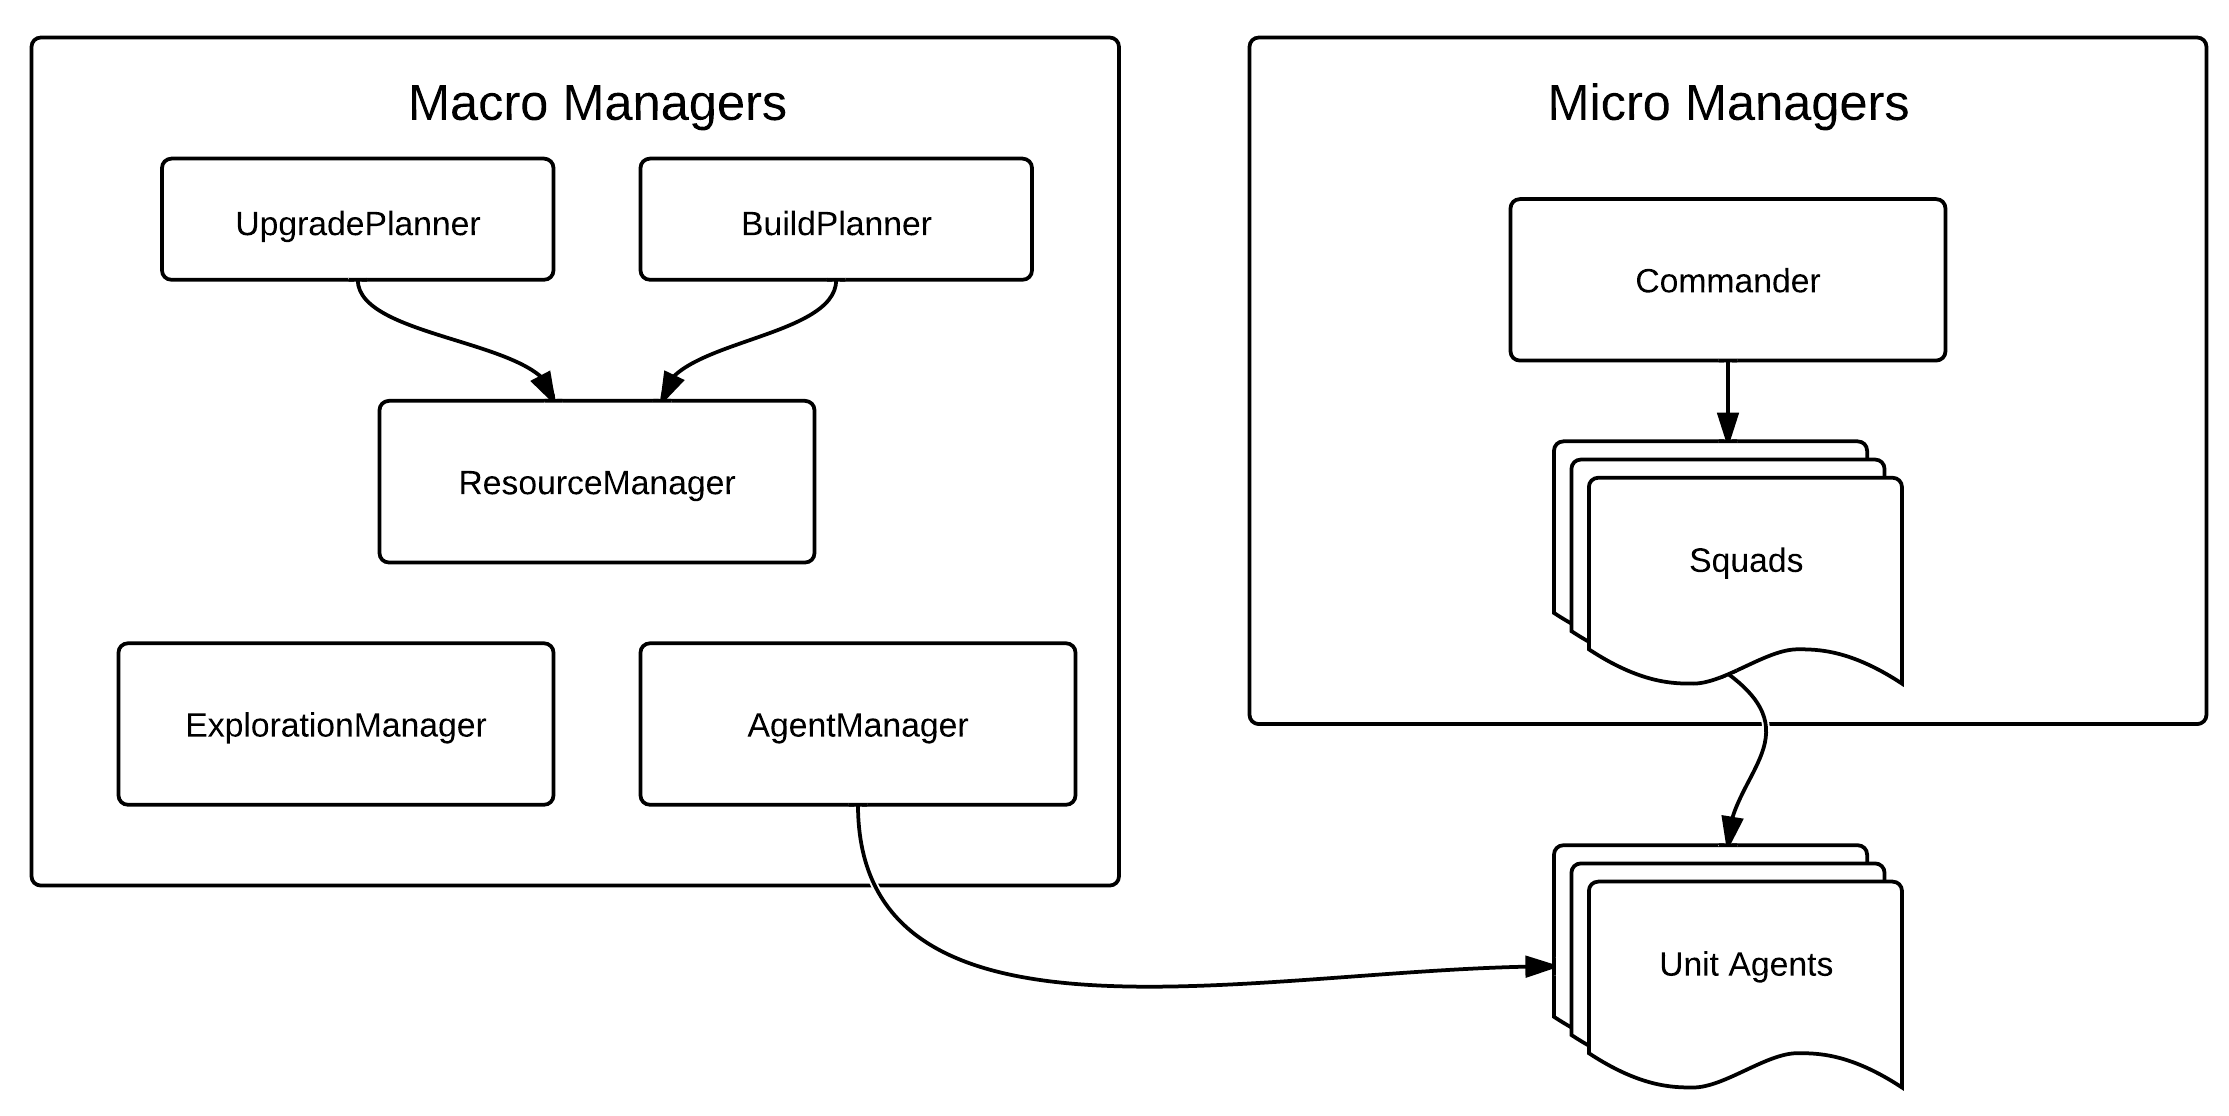
\includegraphics[scale=0.8]{graphics/bthai.png}
\caption{BTHAI general architecture}
\label{fig:bthaiarch}
\end{figure}

\subsubsection{BroodwarBotQ}
Also separates the hierarchy of modules into two levels for micro- and
macro-level management. Instead of letting any of those layers dictate any of
the other, however, it has an arbitrator on top of the hierarchy, that meddles
between the other modules.

\subsubsection{Skynet}
Three-layered architecture, with high-level modules on top, issueing commands
to the modules in the tactics-level, who in turn dispatch tasks to a task
manager which hands the tasks of to the appropriate low-level
(micro-manageing) task handler.

\subsubsection{SPAR}
High-level modules decide which strategies to implement and abstract actions
are dispatched from the module responsible for tactical decisions, while
lower-level modules resolve and execute the detailed steps needed for the
abstract actions.

\subsection{Blackboard Architectures}
Blackboard architectures don't necessarily need a hierarchy of modules, each
module is responsible for interpreting the data in the shared memory itself,
and putting back out the results of processing (if any).

\subsubsection{Nova}
It has three sets of modules; a set of micro-management modules for handling
individual actions, a set of macro-management modules for handling higher-level
planning, economy and production, and finally a single ``strategy manager''
module that is responsible for selecting strategies.

\section{Cognitive Architectures}
Cognitive architectures are architectures that base themselves on some model of
human cognition. There are several competing models of cognition, and one of
the most recent and well-supported is the Global Workspace Theory.

There currently have been no attempts at utilizing cognitive models for playing
Starcraft: BroodWar.

\subsection{Models of cognition}
A cognitive model is an approximation of how cognitive processes work. They are
often used for understanding how humans take decisions, and predict 

\subsection{Global Workspace Theory}

Global Workspace Theory is a model of cognition that is very well supported
by experimental data and has been used to implement processes that imitate
human decision making (for example for solving the problem of assigning
people to jobs in the US Navy). 

It is based around an understanding of the brain as a set of many more or less
independent modules, working together by utilizing a shared workspace (hence the
``global workspace''), and cycles of the various submodules competing for a
space in this shared workspace.\cite{baars2005gwd}

\subsection{Cognitive Models in game AIs}
There have been several more or less successful attempts at implementing models
of cognition into game-playing agents. One of the more recent ones is
CERA-CRANIUM.


\subsection{CERA-CRANIUM}
CERA-CRANIUM intends to implement a general architecture for agents based on
various cognitive architectures, and not tied to any specific model of
cognition. It has already been used to implement a bot that plays Unreal
Tournament 2004 (a first-person shooter game) using a model based on the Global
Workspace Theory, as well as a robot for mapping out an unknown environment.
\cite{arrabales2009ceracranium}

It is based on two major modules:
\begin{description}
 \item [CRANIUM] (Cognitive Robotics Architecture Neurologically Inspired
Underlying Manager) is a tool to create and manage a large amount of
simultanous processes interacting through a shared workspace.
 \item [CERA] (Conscious and Emotional Reasoning Architecture)
 utilizes CRANIUM to create a dynamic control architecture structured in
layers, based on computational models of consciousness.
\end{description}

\subsubsection{CRANIUM}
CRANIUM is basically a software library that can execute thousand of parallel
but coordinated processes.
It is based on the understanding of how the brain works, where specialized
regions process information both from the senses and from other regions, and
the connections between these areas enables the emergence of the global
coordination we see in the brain.\cite{baars2005gwd}

In CRANIUM the various processes/modules are similar to the \textit{demons} in
Dennett's 1992 paper ``Consciousness Explained'', and CRANIUM itself is similar
to a \textit{pandemonium}\cite{dennet1992consciousness}.

The way the various processes collaborate on a shared workspace, by subscribing
to it, then read specific data from it, processing it and finally submitting the
new data back to the workspace is basically a blackboard
system.\cite{nii1986blackboard}

\subsubsection{CERA}
CERA is based around four layers; the sensory-motor services, physical layer,
mission-specific layer and the core layer, based on the services provided by
CRANIUM.

The sensory-motor layer is the most basic, and lowest-level layer, which
provides a uniform interface for sensory input and motoric actuation, physical
or simulated. Each sensor and motor has a service in this layer.

The physical layer wraps the sensory-motor layer, doing some pre-processing of
the sensory data, checking that actuator commands are within safety limits,
etc. It doesn't do semantic information binding, only simple, ``dumb''
pre-processing, though.

The mission-specific layer processes the data from the physical layer,
according to the current missions and sub-goals of those missions, as well as
vital behaviour of the bot (the inherent goals). The strict layering means that
this layer can be modified indendently of the other layers, to account for
various needs depending on the assigned tasks, and accounting for functional
integrity.

The core layer is the highest level, and perform higher cognitive functions,
and it is this layer that is adjusted to implement various cognitive
architectures. It has five core modules, however; attention, status assessment,
preconscious management, memory management and self-coordination. While these
are defined as core modules in CERA, the modular design means that they can be
replaced by a custom set.

The physical and mission-specific layers are inspired by cognitive models of
consciousness, where the various modules compete and collaborate in a shared
workspace. In CERA there is two workspaces; one for searching for the solution
to ``what must be the next content of the agent's conscious perception?'' and
``what must be the next action to execute?''. This differs from traditional AI
control architectures where one only attempts to find the best solution to the
second question, and ignoring the first. \cite{arrabales2009ceracranium} argues
that to successfully answer the second question in a human-like fashion, you
first need to answer the first one.

\subsubsection{Perceptual flow}
Perceptual flow is bottom-up, going from the physical sensors to the CERA core
layer. There are several types of percepts, depending on the level they are
produced in. The \textit{single percepts} are singular quantums of perceptions
directly from the percept pre-processors in the sensor service, \textit{complex
percepts} which are made from several individual single percepts, aggregated by
so-called ``percept aggregators''. These are specialized processors in the
physical layer who are responsible for noticing relations and contexts between
individual single percepts. These two types of percepts are both originating
from processors in the physical layer. From the specialized processors in the
mission-specific layer we get more abstract and complex percepts, who are also
more implementation specific. Some of the most important ones are
\textit{mission percepts}, \textit{complex percepts}, \textit{mismatch
percepts} and \textit{novelty percepts}, which say something about contexts for
the current focus of attention, activation, if some sensors input is not
matching the expected input, and the novelty of certain input.

Single percepts are published to the physical workspace, while combined, complex
percepts are published both to the physical workspace as well as the
mission-specific one, which means it becomes available to the specialized
processors in both layers immediately.

The percepts generated by the processors in the mission-specific layers
get published both to the mission-specific layer, as well as sent to the CERA
core layer. While using a single workspace would be possible, this decoupling
allows for a more modular and general design, where more of the architecture
can be re-used for different problems.

\subsubsection{Action flow}
Action flow is similar to perceptual flow, in that it gets conceptually simpler
the lower you go, and more complex and abstract further up in towards the core
layer. The flow is however top-down. From the processes in the mission-specific
layer comes \textit{mission behaviours}, which are decomposed into
\textit{simple behaviours} by action planners in the physical layer. These are
in turn unpacked into \textit{single actions}, by action pre-processors, which
can be executed by the motor services in the sensory-motor layer.

In the physical layer there is a action dispatcher, which is responsible for
dispatching individual actions to the motor services, according to the order
they come in, and the priority they are assigned from the processors they
originate in; as an example actions from simple behaviours with the highest
priority is executed before other actions from simple behaviours with lower
priority.

The selection of behaviours in the mission-specific layer is in turn controlled
by the core layer, and by mission goals.

\subsubsection{Feedback loops}
Looking at how percepts flow upwards from the sensory-motor layer, and back
down again, we can get a concept of \textit{feedback loops}, where different
kinds of events bounces from different layers in the system.

A feedback loop that only goes to the physical layer is compared to a reflexive
action, while loops that go through to the mission-specific layer and the core
layer respectively are compared to unconsciously performed actions and
higher-level conscious actions.

\subsubsection{Software architecture}
This model has a strong requirement on concurrency and asynchronous input and
output, and the software architecture reflects this. It is based on the
Microsoft Robotics Developer Studio, and the Concurrency and Coordination
Runtime in that, as well as the Decentralized Software Services, to implement a
light-weight distributed service-oriented architecture.

\subsubsection{Knowledge representation}
According to Arrabales\cite{arrabales2009ceracranium}, one of the key problems
in artificial general intelligence is knowledge representation. In CERA-CRANIUM
the knowledge is iteratively processed from the lower levels up to the core
layer, where lower layers contextualize and correlate input for higher level
processes. There is for example a proprioception module \footnote{Proprieception
is the knowledge of relative positions of ones own limbs.} which calculates the
position of exteroceptive sensors (sensors that observe external stimuli).
Knowledge is represented internally by geometrical vectors or integer variables,
referenced by contextual parameters referred to as $J$. Each percept is given a
$J$-index to define the relevant context it pertains to (for example geometric
position, or temporal position).

Handling conflicting and contradictory knowledge (which is very common in not
fully observable scenarious, with for example error-prone sensors) is given two
options; either assigning levels of confidence to the data itself and the
contextual parameters, or generating complex percepts representing the mismatch.

\subsubsection{Workspace modulation}
The core layer and the other layers are linked by the way which the
core layer can adjust the parameters by which the workspaces work. CRANIUM
creates a neural-like environment in which several processes can collaborate
and work towards a common goal, while CERA structures and controls the
collaboration in CRANIUM according to the cognitive architecture it models.

\subsubsection{Activation levels}
Cognitive architectures have a clear distinction betweeen implicit and explicit
processing\cite{atkinson2000consciousness}, and in CERA-CRANIUM all percepts
are by default implicit and get processed unconsciously. A specialized
competition inspired by the pandemonium model mentioned earlier selects the
conscious focus for explicit reasoning. The pandemonium demons are the
percepts, behaviours as well as the specialized processors. These are
constantly assigned an \textit{activation level} by the workspace, based on
input from the core layer.

The activation level is first used to weed out percepts with low activation
levels (to conserve computational power), and then the percepts with the highest
values are iteratively processed until one of them wins, and is selected as
conscious focus.

The specialized processors themselves are assigned more or less computational
power depending on their activation level. For specialized processors the
activation level is based on what input they can process.

At any given time there's also several different behaviours generated, and only
the ones with the highest activation level will be selected and executed.

\subsubsection{Contextualization}
The most important factor for the activation level for behaviours and percepts
is the contextualization criteria, which depends on a $J$-index sent to the
workspace from the core layer. The closer a behaviour or percepts own $J$-value
is to the current context $J$ from the core layer, the higher the activation
parameter it gets assigned. This means that percepts that are close to the
current context, and probably relevant for the problem at hand, will be more
likely to get chosen, and that behaviours that are directed at the current
context focus also will be more likely to be chosen.

Since the contextual bias influences which percepts are created, the perception
process is a very dynamic and active process, and not just a passive data
storage system.

\subsubsection{The Match/Mismatch/Novelty mechanism}
It also uses a mechanism to identify unexpected percepts, expected percepts and
novel percepts, and assigns higher activation values to these. This mechanism
was described by Pentti O. Haikonen in his 2007 book ``Robot Brains: Circuits
and Systems for Conscious Machines''\cite{haikonen2007robotbrains}. As an
example; a percept that doesn't match the predicted data will generate a
mismatch percept with an assigned high activation level because it might
require conscious attention. The core layer can then send a context command
with the appropriate $J$ context index to the workspaces to focus on the
unexpected percept.

\subsubsection{Core layer design}
One of the design goals of CERA-CRANIUM is that the higher cognitive abilities
should be problem domain independent.\cite{arrabales2009ceracranium} This means
that the core-layer is directed by meta-goals, instead of mission-specific ones.
This in turn means that different cognitive architectures (as in the models of
cognition, not software architectures) can be implemented on top of CERA-CRANIUM
in the core layer without having to change the lower levels. An example given by
Arrabales of a meta-goal is discovering abstractions, defined as detecting an
invariant in a variance.

\subsubsection{Goals}
Looking back at the different types of feedback loops (reflexive, unconscious,
and conscious), Arrabales identifies three types of goals;
\textit{basic-goals}, \textit{mission-goals} and \textit{meta-goals}, which are
achieved by their respective loops. While the basic and mission goals can be
kept constant for various cognitive architectures, the meta goals are dependent
on what kind of cognitive architecture the core layer is based on. The core
layer is therefore suited to model in higher cognitive features like emotions,
attention and imagination.

As an example, Arrabales implemented a core layer that continously calculates
a $J$-index and sends it with context commands to the workspaces to direct the
conscious focus. He relates this to the General Workspace Theory, where the
contexts generated are the outlines of the metaphorical ``spotlight'', and to
the Multiple Draft Model, where the core layer is in charge of selecting the
winning version, defined as the reduced set of percepts. His implementation is
rule based, where a set of rules takes in percepts and generates a new
$J$-index. These rules are based on the \textit{meta-goals}, and should
therefore, as explained earlier, be mission and domain independent.